\documentclass{chi2012}

\usepackage{graphics}
\usepackage{times}
% To make various LaTeX processors do the right thing with page size.
\special{papersize=8.5in,11in}
\setlength{\paperheight}{11in}
\setlength{\paperwidth}{8.5in}
\setlength{\pdfpageheight}{\paperheight}
\setlength{\pdfpagewidth}{\paperwidth}
\usepackage[pdftex]{hyperref}
\hypersetup{%
pdftitle={Your Title},
pdfauthor={Your Authors},
pdfkeywords={your keywords},
bookmarksnumbered,
pdfstartview={FitH},
colorlinks,
citecolor=black,
filecolor=black,
linkcolor=black,
urlcolor=black,
breaklinks=true,
}

%\pagenumbering{arabic}  % Arabic page numbers for submission.  Remove this line to eliminate page numbers for the camera ready copy

\begin{document}

% Use this command to override the default ACM copyright statement
% (e.g. for preprints). Remove for camera ready copy.
% \toappear{Submitted for review to CHI 2012.}

\title{SIGCHI Conference Proceedings Format Sample File}
\numberofauthors{2}
\author{
  \alignauthor First Author Name (Blank if Blind Review)\\
    \affaddr{Affiliation (Blank if Blind Review)}\\
    \affaddr{Address (Blank if Blind Review)}\\
    \email{e-mail address (Blank if Blind Review)}\\
    \affaddr{Optional phone number  (Blank if Blind Review)}
  \alignauthor Second Author Name (Blank if Blind Review)\\
    \affaddr{Affiliation (Blank if Blind Review)}\\
    \affaddr{Address (Blank if Blind Review)}\\
    \email{e-mail address (Blank if Blind Review)}\\
    \affaddr{Optional phone number  (Blank if Blind Review)}
}

\maketitle

\begin{abstract}
In this paper we describe the formatting requirements for
SIGCHI Conference Proceedings, and offer recommendations
on writing for the worldwide SIGCHI readership.  Please
review this document even if you have submitted to SIGCHI
conferences before, for some format details have changed
relative to previous years. These include the formatting
of table captions, the formatting of references, and a
requirement to include ACM DL indexing information.
\end{abstract}

\keywords{Guides, instructions, author's kit, conference publications.}

\category{H.5.m.}{Information Interfaces and Presentation
  (e.g. HCI)}{Miscellaneous}

\terms{See list of the limited ACM 16 terms in the instructions, see
  {\small\url{http://www.sheridanprinting.com/sigchi/generalterms.htm}}.
}

\section{Introduction}

This format is to be used for submissions that are
published in the conference proceedings.  We wish to give
this volume a consistent, high-quality appearance. We
therefore ask that authors follow some simple
guidelines. In essence, you should format your paper
exactly like this document. The easiest way to do this is
simply to download a template from the conference web
site, and replace the content with your own material. The
template file contains specially formatted styles (e.g.,
Normal, \texttt{Heading}, \texttt{Bullet}, \texttt{Table
  Text}, \texttt{References}, \texttt{Title},
\texttt{Author}, \texttt{Affiliation}) that will reduce
your work in formatting your submission.

\section{Page Size and Columns}

On each page your material (not including the page number) should fit
within a rectangle of 18 x 23 cm (7 x 9 in.), centered on a US
letter page, beginning 1.9 cm (.75 in.) from the left of the page, with
a .85 cm (.33 in.) space between two 8.4 cm (3.3 in.) columns.  On an
A4 page, use a text area of the same dimensions (18 x 23 cm.), again
centered.  Right margins should be justified, not ragged. Beware,
especially when using this template on a Macintosh, Word can change
these dimensions in unexpected ways.

\section{Typeset Text}

Prepare your submissions on a word processor or typesetter.  Please
note that page layout may change slightly depending upon the printer
you have specified.  For this document, printing to Adobe Acrobat PDF
Writer was specified.  In the resulting page layout,
Figure~\ref{fig:figure1} appears at the top of the left column on page
\pageref{fig:figure1}, and Table~\ref{tab:table1} appears at the top
of the right column on page \pageref{tab:table1}.  You may need to
reposition the figures if your page layout or PDF-generation software
is different.

\subsection{Title and Authors}

Your paper's title, authors and affiliations should run across the
full width of the page in a single column 17.8 cm (7 in.) wide.  The
title should be in Helvetica 18-point bold; use Arial if Helvetica is
not available.  Authors' names should be in Times Roman 12-point bold,
and affiliations in Times Roman 12-point (note that Author and
Affiliation are defined Styles in this template file).

To position names and addresses, use a single-row table with invisible
borders, as in this document.  Alternatively, if only one address is
needed, use a centered tab stop to center all name and address text on
the page; for two addresses, use two centered tab stops, and so
on. For more than three authors, you may have to place some address
information in a footnote, or in a named section at the end of your
paper. Please use full international addresses and telephone dialing
prefixes.  Leave one 10-pt line of white space below the last line of
affiliations.

\subsection{Abstract and Keywords}

Every submission should begin with an abstract of about 150 words,
followed by a set of keywords. The abstract and keywords should be
placed in the left column of the first page under the left half of the
title. The abstract should be a concise statement of the problem,
approach and conclusions of the work described.  It should clearly
state the paper's contribution to the field of HCI.

The first set of keywords will be used to index the paper in the
proceedings. The second set are used to catalogue the paper in the ACM
Digital Library. The latter are entries from the ACM Classification
System~\cite{acm_categories}.  In general, it should only be necessary
to pick one or more of the H5 subcategories, see
\url{http://www.acm.org/class/1998/ccs98.html}

\subsection{Normal or Body Text}

Please use a 10-point Times Roman font or, if this is unavailable,
another proportional font with serifs, as close as possible in
appearance to Times Roman 10-point. The Press 10-point font available
to users of Script is a good substitute for Times Roman. If Times
Roman is not available, try the font named Computer Modern Roman. On a
Macintosh, use the font named Times and not Times New Roman. Please
use sans-serif or non-proportional fonts only for special purposes,
such as headings or source code text.

\subsection{First Page Copyright Notice}

Leave 3 cm (1.25 in.) of blank space for the copyright notice at the
bottom of the left column of the first page. In this template a
floating text box will automatically generate the required space. Note
however that the text box is anchored to the \textbf{ABSTRACT}
heading, so if that heading is deleted the text box will disappear as
well.

\subsection{Subsequent Pages}

On pages beyond the first, start at the top of the page and continue
in double-column format.  The two columns on the last page should be
of equal length.

\begin{figure}
\centering
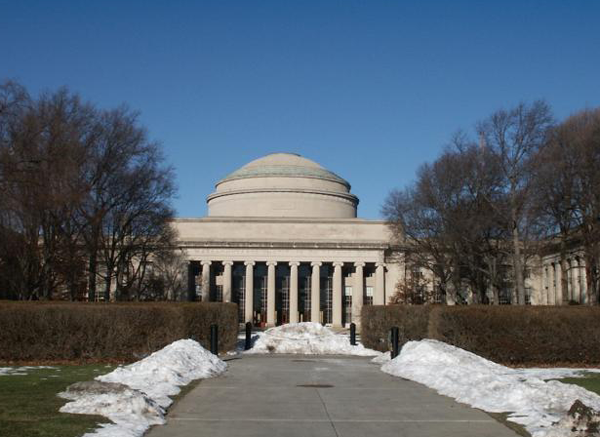
\includegraphics[width=0.9\columnwidth]{Figure1}
\caption{With Caption Below, be sure to have a good resolution image
  (see item D within the preparation instructions).}
\label{fig:figure1}
\end{figure}

\subsection{References and Citations}

Use a numbered list of references at the end of the article, ordered
alphabetically by first author, and referenced by numbers in brackets
\cite{ethics,
  Klemmer:2002:WSC:503376.503378,
  Mather:2000:MUT,
  Zellweger:2001:FAO:504216.504224}. For
papers from conference proceedings, include the title of the paper and
an abbreviated name of the conference (e.g., for Interact 2003
proceedings, use \textit{Proc. Interact 2003}). Do not include the
location of the conference or the exact date; do include the page
numbers if available. See the examples of citations at the end of this
document. Within this template file, use the \texttt{References} style
for the text of your citation.

Your references should be published materials accessible to the
public.  Internal technical reports may be cited only if they are
easily accessible (i.e., you provide the address for obtaining the
report within your citation) and may be obtained by any reader for a
nominal fee.  Proprietary information may not be cited. Private
communications should be acknowledged in the main text, not referenced
(e.g., ``[Robertson, personal communication]'').

\begin{table}
  \begin{tabular}{|c|c|c|}
    \hline
    \bf Objects & 
    \multicolumn{1}{|p{0.3\columnwidth}|}{
      \raggedright \bf Caption --- pre-2002} &
    \multicolumn{1}{|p{0.4\columnwidth}|}{
      \raggedright \bf Caption --- 2003 and afterwards} \\
    \hline
    Tables & Above & Below \\
    \hline
    Figures & Below & Below \\
    \hline
  \end{tabular}
  \caption{Table captions should be placed below the table.}
  \label{tab:table1}
\end{table}

\section{sections}

The heading of a section should be in Helvetica 9-point bold, all in
capitals (\texttt{Heading 1} Style in this template file).  Use Arial
if Helvetica is not available. Sections should not be numbered.

\subsection{Subsections}

Headings of subsections should be in Helvetica 9-point bold with
initial letters capitalized (\texttt{Heading 2}). (Note: For
sub-sections and sub-subsections, a word like \emph{the} or \emph{of}
is not capitalized unless it is the first word of the heading.)

\subsubsection{Sub-subsections}

Headings for sub-subsections should be in Helvetica 9-point italic
with initial letters capitalized (\texttt{Heading 3}).

\section{FIGURES/CAPTIONS}

Place figures and tables at the top or bottom of the appropriate
column or columns, on the same page as the relevant text
(see Figure~\ref{fig:figure1}). A figure or table may extend across both
columns to a maximum width of 17.78 cm (7 in.).

Captions should be Times New Roman 9-point bold (Caption Style in this
template file).  They should be numbered (e.g.,
``Table~\ref{tab:table1}'' or ``Figure~\ref{fig:figure2}''), centered
and placed beneath the figure or table.  Please note that the words
``Figure'' and ``Table'' should be spelled out (e.g., ``Figure''
rather than ``Fig.'') wherever they occur.

Papers and notes may use color figures, which are included in the page
limit; the figures must be usable when printed in black and white in
the proceedings.  The paper may be accompanied by a short video figure
up to five minutes in length.  However, the paper should stand on its
own without the video figure, as the video may not be available to
everyone who reads the paper.

\begin{figure}[h]
\centering

\includegraphics[width=0.9\columnwidth]{Figure2}
\caption{With Caption Below}
\label{fig:figure2}
\end{figure}

\subsection{Inserting Images}

Occasionally MS Word generates larger-than-necessary PDF files when
images inserted into the document are manipulated in MS Word.  To
minimize this problem, use an image editing tool to resize the image
at the appropriate printing resolution (usually 300 dpi), and then
insert the image into Word using Insert | Picture | From File\ldots

\subsection{Table Style}

The text of tables will format better if you use the special
\texttt{Table Text} style (in this template file).  If you do not use
this style, then you may want to adjust the vertical spacing of the
text in the tables. (In Word, use Format | Paragraph\ldots and then
the Line and Page Breaks tab.  Generally, text in each field of a
table will look better if it has equal amounts of spacing above and
below it, as in Table~\ref{tab:table1}.)

\section{LANGUAGE, STYLE AND CONTENT}

The written and spoken language of SIGCHI is English. Spelling and
punctuation may use any dialect of English (e.g., British, Canadian,
US, etc.) provided this is done consistently. Hyphenation is
optional. To ensure suitability for an international audience, please
pay attention to the following: 

\begin{itemize}
\item Write in a straightforward style.
\item Try to avoid long or complex sentence structures.
\item Briefly define or explain all technical terms that may be
  unfamiliar to readers.
\item Explain all acronyms the first time they are used in your text
  --- e.g., ``Digital Signal Processing (DSP)''.
\item Explain local references (e.g., not everyone knows all city
  names in a particular country).
\item Explain ``insider'' comments. Ensure that your whole audience
  understands any reference whose meaning you do not describe (e.g.,
  do not assume that everyone has used a Macintosh or a particular
  application).
\item Explain colloquial language and puns. Understanding phrases like
  ``red herring'' may require a local knowledge of English.  Humor and
  irony are difficult to translate.
\item Use unambiguous forms for culturally localized concepts, such as
  times, dates, currencies and numbers (e.g., ``1-5- 97'' or ``5/1/97''
  may mean 5 January or 1 May, and ``seven o'clock'' may mean 7:00 am or
  19:00).  For currencies, indicate equivalences --- e.g., ``Participants
  were paid 10,000 lire, or roughly \$5.''
\item Be careful with the use of gender-specific pronouns (he, she)
  and other gendered words (chairman, manpower, man-months). Use
  inclusive language that is gender-neutral (e.g., she or he, they,
  s/he, chair, staff, staff-hours,
  person-years). See~\cite{Schwartz:1995:GBF} for further advice and
  examples regarding gender and other personal attributes.
\item If possible, use the full (extended) alphabetic character set
  for names of persons, institutions, and places (e.g.,
  Gr{\o}nb{\ae}k, Lafreni\'ere, S\'anchez, Universit{\"a}t,
  Wei{\ss}enbach, Z{\"u}llighoven, \r{A}rhus, etc.).  These characters
  are already included in most versions of Times, Helvetica, and Arial
  fonts.
\end{itemize}

\section{PAGE NUMBERING, HEADERS AND FOOTERS}

Please submit your anonymous version for reviewing with page numbers
centered in the footer.  These must be removed in the final version of
accepted papers, as page numbers, headers, and footers will be added
by the conference printers.

\section{PRODUCING AND TESTING PDF FILES}

We recommend that you produce a PDF version of your submission well
before the final deadline.  Besides making sure that you are able to
produce a PDF, you will need to check that (a) the length of the file
remains within the submission category's page limit, (b) the PDF file
size is 4 megabytes or less, and (c) the file can be read and printed
using Adobe Acrobat Reader.

Test your PDF file by viewing or printing it with the same software we
will use when we receive it, Adobe Acrobat Reader Version 7. This is
widely available at no cost from~\cite{acrobat}.  Note that most
reviewers will use a North American/European version of Acrobat
reader, which cannot handle documents containing non-North American or
non-European fonts (e.g. Asian fonts).  Please therefore do not use
Asian fonts, and verify this by testing with a North American/European
Acrobat reader (obtainable as above). Something as minor as including
a space or punctuation character in a two-byte font can render a file
unreadable.

\section{BLIND REVIEW}

For archival submissions, CHI requires a ``blind review.'' To prepare
your submission for blind review, remove author and institutional
identities in the title and header areas of the paper. You may also
need to remove part or all of the Acknowledgments text.  Further
suppression of identity in the body of the paper and references is
left to the authors' discretion. For more details, see the submission
guidelines and checklist for your submission category.

\section{CONCLUSION}

It is important that you write for the SIGCHI audience.  Please read
previous years' Proceedings to understand the writing style and
conventions that successful authors have used.  It is particularly
important that you state clearly what you have done, not merely what
you plan to do, and explain how your work is different from previously
published work, i.e., what is the unique contribution that your work
makes to the field?  Please consider what the reader will learn from
your submission, and how they will find your work useful.  If you
write with these questions in mind, your work is more likely to be
successful, both in being accepted into the Conference, and in
influencing the work of our field.

\section{ACKNOWLEDGMENTS}

We thank CHI, PDC and CSCW volunteers, and all publications support
and staff, who wrote and provided helpful comments on previous
versions of this document.  Some of the references cited in this paper
are included for illustrative purposes only.

\balancecolumns
\bibliographystyle{acm-sigchi}
\bibliography{sample2}

\end{document}

